\documentclass{standalone}
\usepackage{tikz}
\usetikzlibrary{patterns, positioning}
\usepackage[sfdefault]{ClearSans} %% option 'sfdefault' activates Clear Sans as the default text font
\usepackage[T1]{fontenc}

\begin{document}
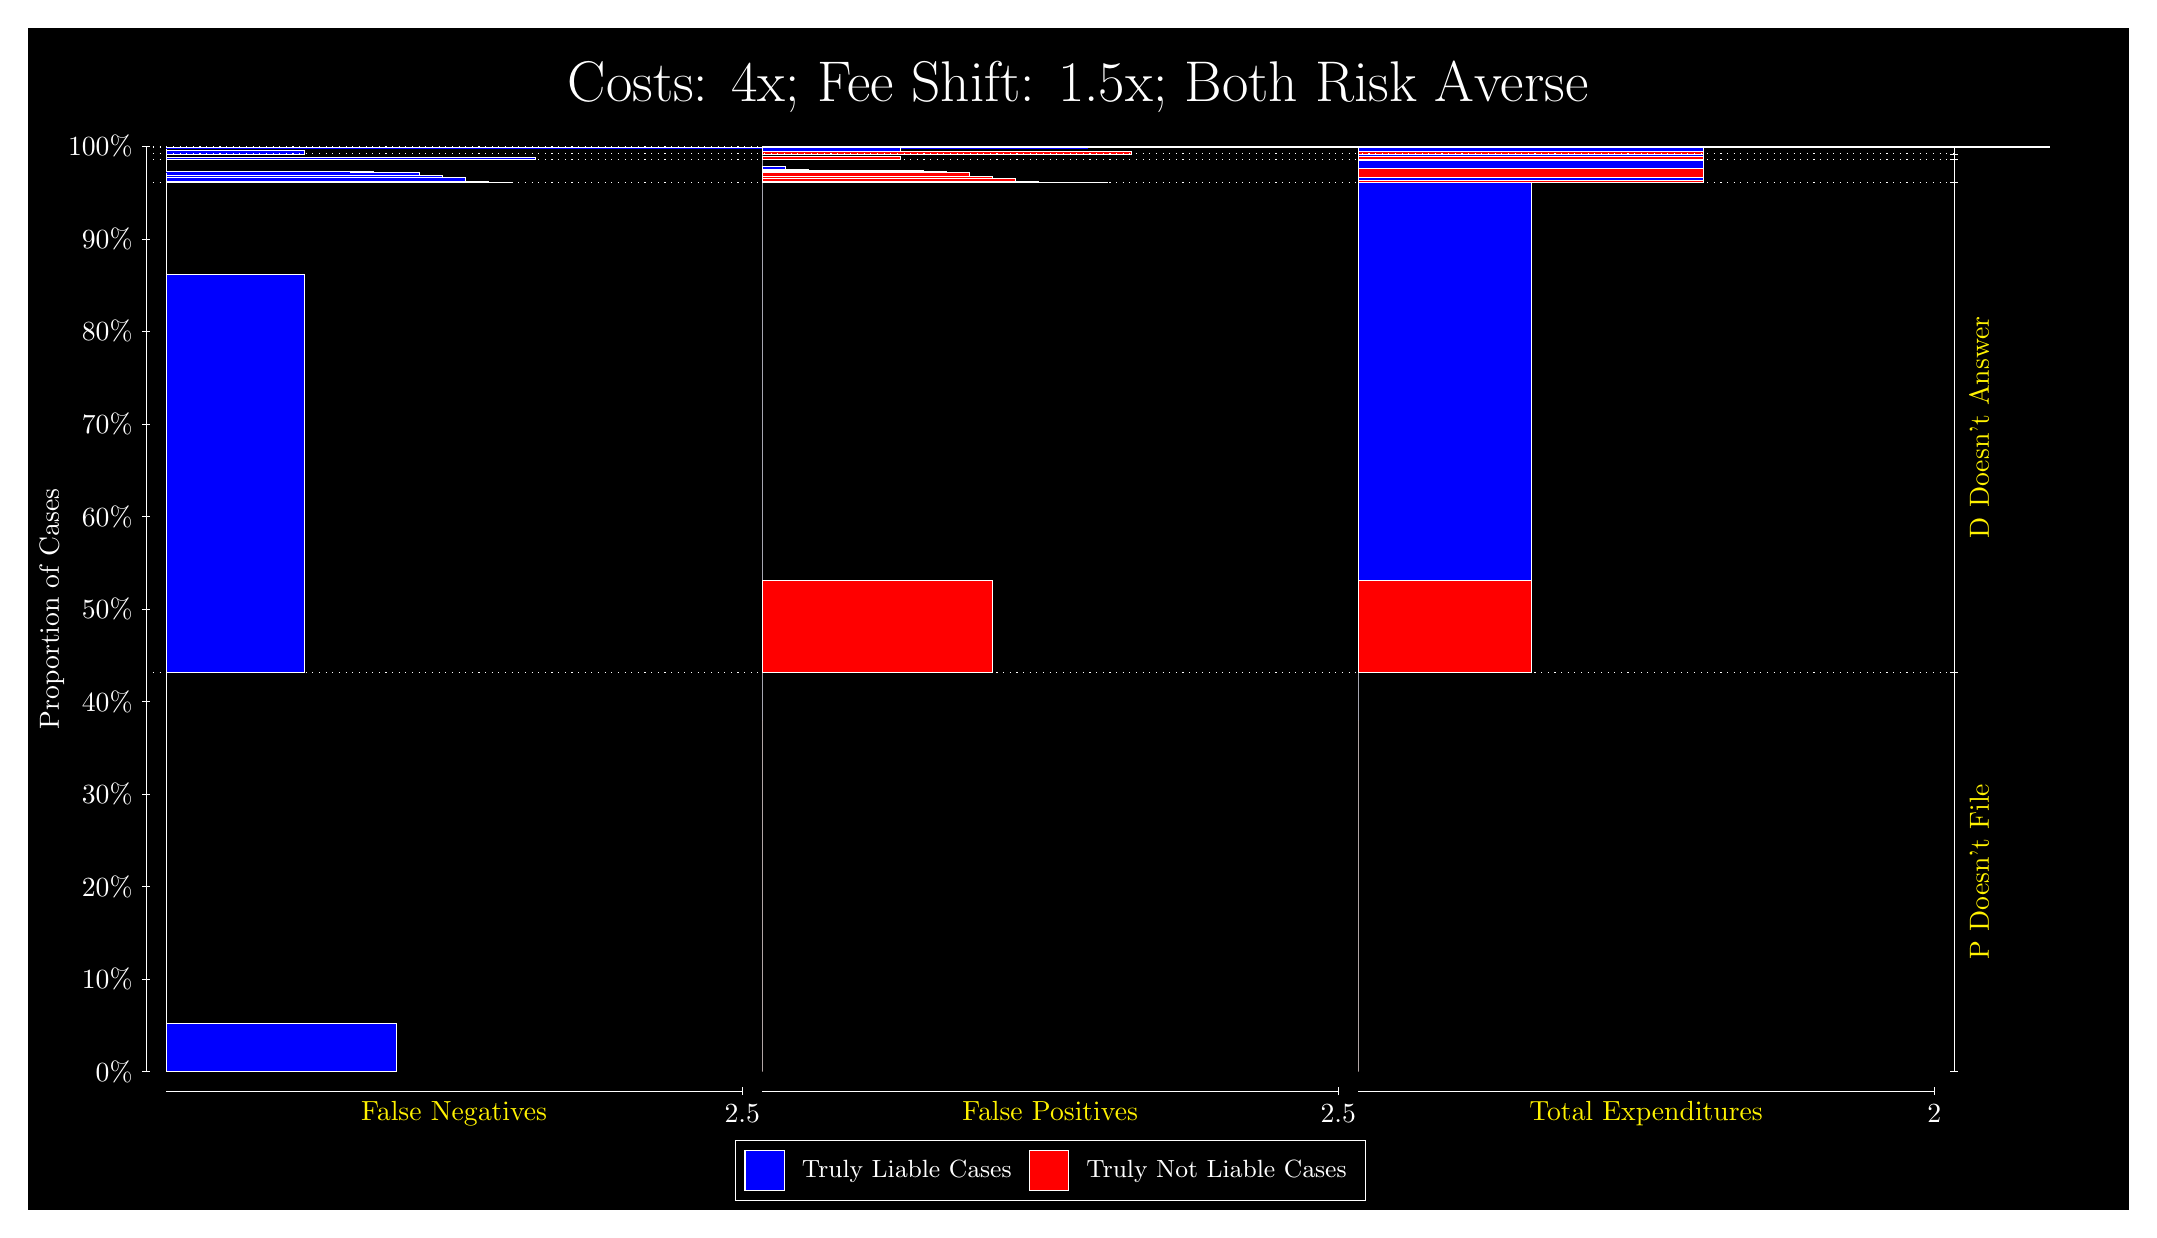
\begin{tikzpicture}
\draw[fill=black] (0,0) rectangle (26.667,15);
\draw[text=white] (0,13.5) rectangle (26.667,15) node[midway] {\huge Costs: 4x; Fee Shift: 1.5x; Both Risk Averse};
\draw[white, very thin] (1.5,1.75) -- (1.5,13.5);
\node[rotate=90, text=white, anchor=center] at (0.3, 7.625) {Proportion of Cases};
\draw[white, very thin] (1.45,1.75) -- (1.55,1.75);
\node[text=white, anchor=east] at (1.45, 1.75) {0\%};
\draw[white, very thin] (1.45,2.925) -- (1.55,2.925);
\node[text=white, anchor=east] at (1.45, 2.925) {10\%};
\draw[white, very thin] (1.45,4.1) -- (1.55,4.1);
\node[text=white, anchor=east] at (1.45, 4.1) {20\%};
\draw[white, very thin] (1.45,5.275) -- (1.55,5.275);
\node[text=white, anchor=east] at (1.45, 5.275) {30\%};
\draw[white, very thin] (1.45,6.45) -- (1.55,6.45);
\node[text=white, anchor=east] at (1.45, 6.45) {40\%};
\draw[white, very thin] (1.45,7.625) -- (1.55,7.625);
\node[text=white, anchor=east] at (1.45, 7.625) {50\%};
\draw[white, very thin] (1.45,8.8) -- (1.55,8.8);
\node[text=white, anchor=east] at (1.45, 8.8) {60\%};
\draw[white, very thin] (1.45,9.975) -- (1.55,9.975);
\node[text=white, anchor=east] at (1.45, 9.975) {70\%};
\draw[white, very thin] (1.45,11.15) -- (1.55,11.15);
\node[text=white, anchor=east] at (1.45, 11.15) {80\%};
\draw[white, very thin] (1.45,12.325) -- (1.55,12.325);
\node[text=white, anchor=east] at (1.45, 12.325) {90\%};
\draw[white, very thin] (1.45,13.5) -- (1.55,13.5);
\node[text=white, anchor=east] at (1.45, 13.5) {100\%};

\draw[white, very thin] (24.457,1.75) -- (24.457,13.5);
\draw[white, very thin] (24.407,1.75) -- (24.507,1.75);
\node[anchor=west] at (24.407, 1.75) {};
\draw[white, very thin] (24.407,6.8229) -- (24.507,6.8229);
\node[anchor=west] at (24.407, 6.8229) {};
\draw[white, very thin] (24.407,13.04) -- (24.507,13.04);
\node[anchor=west] at (24.407, 13.04) {};
\draw[white, very thin] (24.407,13.334) -- (24.507,13.334);
\node[anchor=west] at (24.407, 13.334) {};
\draw[white, very thin] (24.407,13.405) -- (24.507,13.405);
\node[anchor=west] at (24.407, 13.405) {};
\draw[white, very thin] (24.407,13.482) -- (24.507,13.482);
\node[anchor=west] at (24.407, 13.482) {};
\draw[white, very thin] (24.407,13.493) -- (24.507,13.493);
\node[anchor=west] at (24.407, 13.493) {};
\draw[white, very thin] (24.407,13.5) -- (24.507,13.5);
\node[anchor=west] at (24.407, 13.5) {};

\draw[white, very thin, fill=blue] (1.75,1.75) rectangle (4.6775,2.36);
\draw[white, very thin, fill=red] (1.75,2.36) rectangle (1.75,6.8229);
\draw[white, very thin, fill=blue] (1.75,6.8229) rectangle (3.5065,11.869);
\draw[white, very thin, fill=red] (1.75,11.869) rectangle (1.75,13.04);
\draw[white, very thin, fill=blue] (1.75,13.04) rectangle (6.1413,13.043);
\draw[white, very thin, fill=blue] (1.75,13.043) rectangle (5.8486,13.056);
\draw[white, very thin, fill=blue] (1.75,13.056) rectangle (5.5558,13.104);
\draw[white, very thin, fill=blue] (1.75,13.104) rectangle (5.2631,13.134);
\draw[white, very thin, fill=blue] (1.75,13.134) rectangle (4.9703,13.167);
\draw[white, very thin, fill=blue] (1.75,13.167) rectangle (4.6775,13.173);
\draw[white, very thin, fill=blue] (1.75,13.173) rectangle (4.3848,13.178);
\draw[white, very thin, fill=blue] (1.75,13.178) rectangle (4.092,13.179);
\draw[white, very thin, fill=blue] (1.75,13.179) rectangle (3.7993,13.181);
\draw[white, very thin, fill=red] (1.75,13.181) rectangle (1.75,13.334);
\draw[white, very thin, fill=blue] (1.75,13.334) rectangle (6.4341,13.363);
\draw[white, very thin, fill=red] (1.75,13.363) rectangle (1.75,13.405);
\draw[white, very thin, fill=blue] (1.75,13.405) rectangle (3.5065,13.446);
\draw[white, very thin, fill=red] (1.75,13.446) rectangle (1.75,13.482);
\draw[white, very thin, fill=blue] (1.75,13.482) rectangle (13.46,13.485);
\draw[white, very thin, fill=red] (1.75,13.485) rectangle (1.75,13.493);
\draw[white, very thin, fill=red] (1.75,13.493) rectangle (1.75,13.495);
\draw[white, very thin, fill=blue] (1.75,13.495) rectangle (1.75,13.5);
\draw[white, very thin, fill=red] (9.3189,1.75) rectangle (9.3189,6.213);
\draw[white, very thin, fill=blue] (9.3189,6.213) rectangle (9.3189,6.8229);
\draw[white, very thin, fill=red] (9.3189,6.8229) rectangle (12.246,7.9936);
\draw[white, very thin, fill=blue] (9.3189,7.9936) rectangle (9.3189,13.04);
\draw[white, very thin, fill=red] (9.3189,13.04) rectangle (13.71,13.041);
\draw[white, very thin, fill=red] (9.3189,13.041) rectangle (13.417,13.042);
\draw[white, very thin, fill=red] (9.3189,13.042) rectangle (13.125,13.047);
\draw[white, very thin, fill=red] (9.3189,13.047) rectangle (12.832,13.054);
\draw[white, very thin, fill=red] (9.3189,13.054) rectangle (12.539,13.089);
\draw[white, very thin, fill=red] (9.3189,13.089) rectangle (12.246,13.12);
\draw[white, very thin, fill=red] (9.3189,13.12) rectangle (11.954,13.171);
\draw[white, very thin, fill=red] (9.3189,13.171) rectangle (11.661,13.186);
\draw[white, very thin, fill=red] (9.3189,13.186) rectangle (11.368,13.194);
\draw[white, very thin, fill=blue] (9.3189,13.194) rectangle (10.783,13.195);
\draw[white, very thin, fill=blue] (9.3189,13.195) rectangle (10.49,13.197);
\draw[white, very thin, fill=blue] (9.3189,13.197) rectangle (10.197,13.201);
\draw[white, very thin, fill=blue] (9.3189,13.201) rectangle (9.9044,13.208);
\draw[white, very thin, fill=blue] (9.3189,13.208) rectangle (9.6116,13.241);
\draw[white, very thin, fill=blue] (9.3189,13.241) rectangle (9.3189,13.334);
\draw[white, very thin, fill=red] (9.3189,13.334) rectangle (11.075,13.376);
\draw[white, very thin, fill=blue] (9.3189,13.376) rectangle (9.3189,13.405);
\draw[white, very thin, fill=red] (9.3189,13.405) rectangle (14.003,13.441);
\draw[white, very thin, fill=blue] (9.3189,13.441) rectangle (11.075,13.482);
\draw[white, very thin, fill=red] (9.3189,13.482) rectangle (9.3189,13.491);
\draw[white, very thin, fill=blue] (9.3189,13.491) rectangle (9.3189,13.493);
\draw[white, very thin, fill=red] (9.3189,13.493) rectangle (21.029,13.495);
\draw[white, very thin, fill=blue] (9.3189,13.495) rectangle (18.102,13.5);
\draw[white, very thin, fill=red] (16.888,1.75) rectangle (16.888,6.213);
\draw[white, very thin, fill=blue] (16.888,6.213) rectangle (16.888,6.8229);
\draw[white, very thin, fill=red] (16.888,6.8229) rectangle (19.083,7.9936);
\draw[white, very thin, fill=blue] (16.888,7.9936) rectangle (19.083,13.04);
\draw[white, very thin, fill=red] (16.888,13.04) rectangle (21.279,13.075);
\draw[white, very thin, fill=blue] (16.888,13.075) rectangle (21.279,13.107);
\draw[white, very thin, fill=red] (16.888,13.107) rectangle (21.279,13.22);
\draw[white, very thin, fill=blue] (16.888,13.22) rectangle (21.279,13.322);
\draw[white, very thin, fill=red] (16.888,13.322) rectangle (21.279,13.328);
\draw[white, very thin, fill=blue] (16.888,13.328) rectangle (21.279,13.334);
\draw[white, very thin, fill=red] (16.888,13.334) rectangle (21.279,13.376);
\draw[white, very thin, fill=blue] (16.888,13.376) rectangle (21.279,13.405);
\draw[white, very thin, fill=red] (16.888,13.405) rectangle (21.279,13.441);
\draw[white, very thin, fill=blue] (16.888,13.441) rectangle (21.279,13.482);
\draw[white, very thin, fill=red] (16.888,13.482) rectangle (25.67,13.491);
\draw[white, very thin, fill=blue] (16.888,13.491) rectangle (25.67,13.493);
\draw[white, very thin, fill=red] (16.888,13.493) rectangle (25.67,13.495);
\draw[white, very thin, fill=blue] (16.888,13.495) rectangle (25.67,13.5);
\draw[white, dotted] (1.5,6.8229) -- (24.457,6.8229);
\draw[white, dotted] (1.5,13.04) -- (24.457,13.04);
\draw[white, dotted] (1.5,13.334) -- (24.457,13.334);
\draw[white, dotted] (1.5,13.405) -- (24.457,13.405);
\draw[white, dotted] (1.5,13.482) -- (24.457,13.482);
\draw[white, dotted] (1.5,13.493) -- (24.457,13.493);
\draw[white, very thin] (1.75,1.5) -- (9.0689,1.5);
\node[text=yellow, anchor=north] at (5.4094, 1.5) {False Negatives};
\draw[white, very thin] (9.0689,1.45) -- (9.0689,1.55);
\node[text=white, anchor=north] at (9.0689, 1.45) {2.5};

\draw[white, very thin] (9.3189,1.5) -- (16.638,1.5);
\node[text=yellow, anchor=north] at (12.978, 1.5) {False Positives};
\draw[white, very thin] (16.638,1.45) -- (16.638,1.55);
\node[text=white, anchor=north] at (16.638, 1.45) {2.5};

\draw[white, very thin] (16.888,1.5) -- (24.207,1.5);
\node[text=yellow, anchor=north] at (20.547, 1.5) {Total Expenditures};
\draw[white, very thin] (24.207,1.45) -- (24.207,1.55);
\node[text=white, anchor=north] at (24.207, 1.45) {2};

\node[text=yellow, centered, rotate=90] at (24.777, 4.2865) {P Doesn't File};
\node[text=yellow, centered, rotate=90] at (24.777, 9.9315) {D Doesn't Answer};






\draw (12.978300999999998,1.5) node[draw=none] (baseCoordinate) {};
\begin{scope}[align=center]
        \matrix[scale=0.5, draw=white, below=0.5cm of baseCoordinate, nodes={draw}, column sep=0.1cm]{
            \node[rectangle, draw, minimum width=0.5cm, minimum height=0.5cm, fill=blue] {}; &
            \node[draw=none, font=\small, text=white] (B) {Truly Liable Cases}; &
            \node[rectangle, draw, minimum width=0.5cm, minimum height=0.5cm, fill=red] {}; &
            \node[draw=none, font=\small, text=white] (B) {Truly Not Liable Cases}; \\
            };
\end{scope}

\end{tikzpicture}
\end{document}